\chapter{Photons generation in coupled resonators}
\begin{figure}[H]
\centering
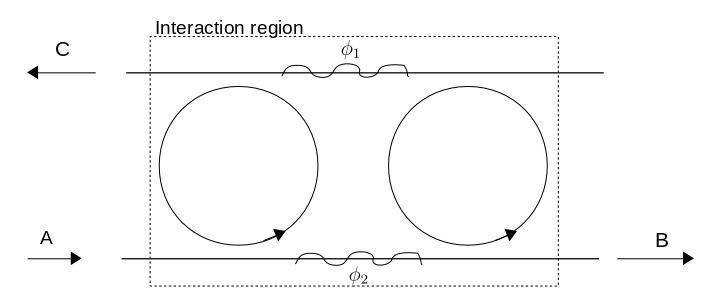
\includegraphics[width = .8\textwidth]{img/system}
\caption{Coupled resonators, Spontaneous Four Wave Mixing happens only inside the rings, there are three channels labelled as A,B, and C}
\label{couplesstructure}
\end{figure}

In this last chapter we study the generation of entangled photons via Spontaneous Four Wave Mixing in the structure of figure \ref{couplesstructure}. As can be seen from figure \ref{couplesstructure}, the structure is composed by two ADF in series, the channel are labelled with the letters $A$, $B$, $C$ and $D$, in this work we assume that the input is in channel $A$ and the output can be in either in $B$ or in $C$. When numerical examples are presented, they will refer to the SOI structures described in chapter 1. The work starts by writing the non-linear Hamiltonian in terms of the asymptotic states developed in section \ref{section:asymptotic}, then we solve the dynamics of the photons state using the backward Heisenberg approach developed in section \ref{heinsemberg} and finally we study the results.
\section{Asymptotic fields}
\begin{figure}[H]
\centering
\begin{subfigure}{0.5\textwidth}
\centering
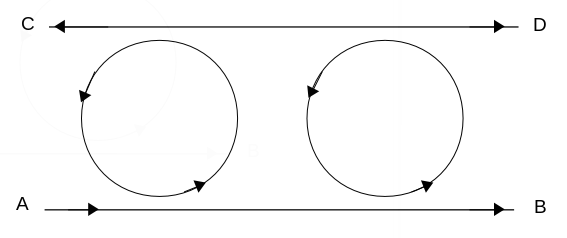
\includegraphics[width = \textwidth]{img/Asyina2}
\caption{Asymptotic in field for channel $A$}
\end{subfigure}%
\begin{subfigure}{0.5\textwidth}
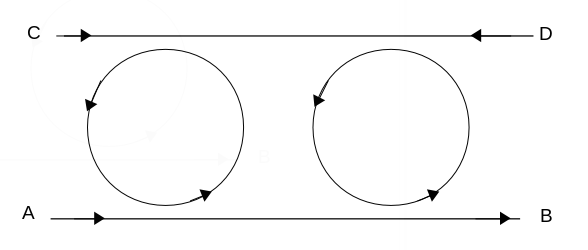
\includegraphics[width = \textwidth]{img/Asyoutb2}
\caption{Asymptotic out field for channel $B$}
\end{subfigure}
\caption{Asymptotic fields for the coupled resonators, the ring on the left is identified as 1, while the ring on the right as 2}\label{asyfields}
\end{figure}
We take as input state a coherent state in channel A, so we can write it as $\ket{\psi_{in}} = e^{\alpha A_p^\dagger - \text{H.c}}\ket{vac}$ where $A_p^\dagger = \int dk \phi_P(k) a_k^\dagger$. The non linear Hamiltonian is \cite{Sipe2004}
\begin{equation}\label{nonlinearhamiltonian}H_{NL} = -\frac{1}{3\varepsilon_0}\int\Gamma^{ijkl}_3(\r)D^iD^jD^kD^l\,d\r\end{equation}
where summation over repeated indexes is implied. Since the asymptotic states are a complete basis we can expand $D$ either on the asympotic-out states, or on the asymptotic-in, we can choose to expand two fields of \eqref{nonlinearhamiltonian} in terms of the asymptotic-in and the other two in terms of the asympotic-out.
Keeping only the Spontaneous Four Wave Mixing terms we arrive at:
\begin{multline}H_{NL} = -\int dk_1dk_2dk_3dk_4S_{bb}(k_1,k_2,k_3,k_4)a_{k_1}a_{k_2}b_{b,k_3}^\dagger b_{b,k_4}^\dagger \\-2\int dk_1dk_2dk_3dk_4S_{bc}(k_1,k_2,k_3,k_4)a_{k_1}a_{k_2}b_{b,k_3}^\dagger b_{c,k_4}^\dagger\\ -\int dk_1dk_2dk_3dk_4S_{cc}(k_1,k_2,k_3,k_4)a_{k_1}a_{k_2}b_{c,k_3}^\dagger b_{c,k_4}^\dagger +\text{H.c.}\end{multline}
where $a_k$ is the annihilation operator associated with channel A, $b_{b,k}$ is for channel B and $b_{c,k}$ refers to channel C and we defined the following quantity
\begin{multline}\label{S}
S_{xy}(k_1,k_2,k_3,k_4) = \frac{3}{2\varepsilon_0}\sqrt{\frac{(\hbar\omega_{k_1})(\hbar\omega_{k_2})(\hbar\omega_{k_3})(\hbar\omega_{k_4})}{16}}\cdot \\ \int d\r \Gamma^{ijkl}_3D^{i,asy-in}_{a,k_1}(\r)D^{j,asy-in}_{a,k_2}(\r)\left[D^{k,asy-out}_{x,k_3}(\r)\right]^*\left[D^{l,asy-out}_{y,k_4}(\r)\right]^*
\end{multline}
we derive now the explicit form of $S_{bb}$ and in analogy also for $S_{bc}$ and $S_{cc}$. In section \ref{section:asymptotic} we stated that the asympotic-in field associated with channel $A$ corresponds to a wave incoming in channel $A$ and outgoing waves in all other channels, and similarly the asymptotic-out field of channel $B$ consists of an outgoing wave in channel $B$ and incoming waves in the other channels. These asymptotic fields are depicted in figure \ref{asyfields}. The integral of $S_{bb}$ is performed in general over all space, but outside the waveguides and resonators the field is zero; furthermore, since the field inside the ring is enhanced with respect to the field in the waveguide, we can neglect the contribution of the field in the waveguides. Therefore the integration can be performed only over the rings. With this assumption we can write the asymptotic fields as
\begin{equation}\mathbf{D}^{asy-in\,(rings)}_{a,k} = FE_{1a}(\omega) \mathbf{d}^1_{k_1}(\r_\perp)e^{ik_1z} + FE_{2a}(\omega) \mathbf{d}_{k_2}^2(\r_\perp)e^{ik_2z} \end{equation}
where $z$ is the coordinate in the counterclockwise direction along the rings circumference and $\r_\perp$ are the coordinates perpendicular to $z$. $FE_{1a}$ is the field enhancement of the first ring when the input wave is in channel $A$, while obviously $FE_{2a}$ refers to the second ring, and $\mathbf{d}^1_{k_1}(\r_\perp)$ is the linear mode profile. Similarly the asymptotic-out field associated with channel $B$ can be written as
\begin{equation}\mathbf{D}^{asy-out\,(rings)}_{b,k} = FE_{1b}(\omega) \mathbf{d}^1_{k_1}(\r_\perp)e^{ik_1z} + FE_{2b}(\omega)\mathbf{d}_{k_2}^2(\r_\perp)e^{ik_2z} \end{equation}
using the last two equations in \eqref{S} leads to a lot of terms, each associated with a specific physical interpretation. In particular every terms correspond to a possible path for the photons that are scattered in the channel $B$: for example, the annihilated pump photons can be both inside the first ring, or both in the second one, or one in the first ring and one in the second one. The same argument holds for the created photons, that can be created both inside the first ring, both inside the second or one in each ring. The combination of these paths are represented by all terms in $S_{bb}$; however, each of these terms are proportional to the field $\mathbf{d}^1_{k_1}(\r_{\perp})$ and $\mathbf{d}^2_{k_2}(\r_{\perp})$ that are non-zero only inside the ring, therefore a term that contains a factor $\mathbf{d}^1_{k_1}(\r_{\perp})\mathbf{d}^2_{k_2}(\r_{\perp})$ is zero everywhere, because in the first ring the second factor is zero and in the second ring the first factor is zero. The only term that survive the integration are those who have all factors equal to  $\mathbf{d}^1_{k_1}(\r_{\perp})$ or $\mathbf{d}^2_{k_2}(\r_{\perp})$, that is only the path where the two pump photons are annihilated in the same ring where the signal and indler photons are created. Therefore we can write $S_{bb}$ as
\begin{multline}S_{bb} =\frac{3}{2\varepsilon_0}\sqrt{\frac{(\hbar\omega_{k_1})(\hbar\omega_{k_2})(\hbar\omega_{k_3})(\hbar\omega_{k_4})}{16}}\cdot\\\Bigg( \int d\r \Gamma^{ijkl}_3FE_{1a}(\omega_1)FE_{1a}(\omega_2)FE^*_{1b}(\omega_3)FE^*_{1b}(\omega_4)d^{1,i}_{k_1}(\r_{\perp})d^{1,j}_{k_2}(\r_{\perp})d^{1,k}_{k_3}(\r_{\perp})d^{1,l}_{k_4}(\r_{\perp})e^{i\Delta k z} +\\
\int d\r \Gamma^{ijkl}_3FE_{2a}(\omega_1)FE_{2a}(\omega_2)FE^*_{2b}(\omega_3)FE^*_{2b}(\omega_4)d^{2,i}_{k_1}(\r_{\perp})d^{2,j}_{k_2}(\r_{\perp})d^{2,k}_{k_3}(\r_{\perp})d^{2,l}_{k_4}(\r_{\perp})e^{i\Delta k z}\Bigg)\end{multline}
where $\Delta k = k_1 + k_2 -k_3 - k_4$. The integration in $z$ can be done easly
\begin{equation}\int_0^{L} e^{i\Delta k z} dz = \frac{1}{i\Delta k}(e^{i\Delta k L} - 1) = \frac{e^{i\Delta k L/2}}{i\Delta k}(e^{i\Delta k L/2}- e^{-i\Delta k L/2}) = \frac{2}{\Delta k}e^{i\Delta k L/2} \sin\left(\Delta k \frac{L}{2}\right)\end{equation}
which can be written as $\frac{L}{\pi}e^{i\Delta k L/2} \text{sinc}\left(\Delta k \frac{L}{2\pi}\right)$. If we define the following
\begin{equation}\gamma_1 = \frac{3}{2\varepsilon_0}\int d\r_\perp \Gamma^{ijkl}_3d^{1,i}_{k_1}(\r_{\perp})d^{1,j}_{k_2}(\r_{\perp})d^{1,k}_{k_3}(\r_{\perp})d^{1,l}_{k_4}(\r_{\perp})\end{equation}
and the related $\gamma_2$, notice that in the case $\mathbf{d}^{1}_{k} = \mathbf{d}^{2}_{k}$, then $\gamma_1 = \gamma_2 \equiv \gamma_{NL}$.  The expression for $S_{bb}$ is finally:
\begin{multline}\label{sbbfinal} S_{bb} = \frac{L}{\pi}e^{i\Delta k L/2} \text{sinc}\left(\Delta k \frac{L}{2\pi}\right) \sqrt{\frac{(\hbar\omega_{k_1})(\hbar\omega_{k_2})(\hbar\omega_{k_3})(\hbar\omega_{k_4})}{16}}\cdot\\ \Bigg( \gamma_1 FE_{1a}(\omega_1)FE_{1a}(\omega_2)FE^*_{1b}(\omega_3)FE^*_{1b}(\omega_4) +\gamma_2 FE_{2a}(\omega_1)FE_{2a}(\omega_2)FE^*_{2b}(\omega_3)FE^*_{2b}(\omega_4)\Bigg)\end{multline}

\section{Output states}
With this expression we can switch to the Heisenberg picture and we can define
\begin{equation}\label{potential}
V(t) = U_L^\dagger H_{NL}U_{L}\end{equation}
since the operator $U_L$ satisfies the unitary relation $U_L U_L^\dagger = U_L^\dagger U_L = \mathbbm{1}$ we can insert $U_L^\dagger U_L$ between every annhilation and creation operators and define the time dependent operator, for example $a_{k}(t) \equiv U_L^\dagger a_{k}U_L$. These operators satisfy the Heisenberg equation
\begin{equation}\frac{da_{k}}{dt} = \frac{1}{i\hbar}[a_{k},H_L]\end{equation}
which we can solve for every operator. For example for $a_{k}$ the commutator with the linear Hamiltonian is:
\begin{equation}[a_{k},H_L] = \int dk'\hbar \omega_{k'}a_{k} a_{k'}^\dagger a_{k'}-\int dk'\hbar \omega_{k'}a_{k'}^\dagger a_{k'}a_{k}\end{equation}
we know that $[a_k,a_{k'}^\dagger] = \delta(k-k')\implies a_{k} a_{k'}^\dagger = \delta(k-k') + a_{k'}^\dagger a_{k}$; substituting this into the first term we arrive at
\begin{equation}[a_{k},H_L] = \int dk'\hbar \omega_{k'}a_{k}\delta(k-k') = \hbar \omega_{k}a_{k}\end{equation}
so the Heisenberg equation can be written as
\begin{equation}\frac{da_{k}}{dt} = -i\omega_{k}a_{k}\end{equation}
which has the trivial solution $a_k(t) = a_k(0)e^{-i\omega_k t}$, since $a_k(0) = a_k$ we can write \eqref{potential} 
\begin{equation}V(t) = V_{bb} + 2V_{bc} + V_{cc}\end{equation}
where
\begin{equation}V_{xy} = -\int dk_1dk_2dk_3dk_4S_{xy}(k_1,k_2,k_3,k_4;t)a_{k_1}a_{k_2}b_{x,k_3}^\dagger b_{y,k_4}^\dagger +\text{H.c} \end{equation}
and $S_{xy}(k_1,k_2,k_3,k_4;t) = S_{xy}(k_1,k_2,k_3,k_4)e^{-i(\omega_{k1}+\omega_{k2}-\omega_{k3}-\omega_{k4})t}$. In a similar way it is possible to construct $\hat{V}(t)$
\begin{equation}\hat{V}(t) = U(t_1,t)V(t)U^\dagger(t_1,t) = \hat{V}_{bb}(t) + 2\hat{V}_{bc}(t) + \hat{V}_{cc}(t)\end{equation}
where 
\begin{equation}\hat{V}_{xy}(t) = -\int dk_1dk_2dk_3dk_4S_{xy}(k_1,k_2,k_3,k_4;t)\overline{a}_{k_1}(t)\overline{a}_{k_2}(t)\overline{b}_{x,k_3}^\dagger(t) \overline{b}_{y,k_4}^\dagger(t) +\text{H.c}\end{equation}
now we have all the elements necessary for integrating the equation \eqref{dynamicO}, we need to solve it for the operator $\overline{a}^\dagger_{k}(t)$
\begin{equation}\label{meinkampf}-i\hbar \frac{d\overline{a}^\dagger_{k}(t)}{dt} = [\overline{a}^\dagger_{k},\hat{V}(t)] = [\overline{a}^\dagger_{k},\hat{V}_{bb}(t)] + [\overline{a}^\dagger_{k},2\hat{V}_{bc}(t)] +[\overline{a}^\dagger_{k},\hat{V}_{cc}(t)]\end{equation}
we must work out the three commutators, they are all similar, so we show only one:
\begin{multline}[\overline{a}^\dagger_{k},\hat{V}_{bb}(t)] = -\int dk_1dk_2dk_3dk_4S_{bb}(k_1,k_2,k_3,k_4;t)\overline{a}^\dagger_{k}(t)\overline{a}_{k_1}(t)\overline{a}_{k_2}(t)\overline{b}_{b,k_3}^\dagger(t) \overline{b}_{b,k_4}^\dagger(t) \\
-\int dk_1dk_2dk_3dk_4S_{bb}(k_1,k_2,k_3,k_4;t)\overline{a}^\dagger_{k}(t)\overline{a}^\dagger_{k_1}(t)\overline{a}^\dagger_{k_2}(t)\overline{b}_{b,k_3}(t) \overline{b}_{b,k_4}(t) \\
+ \int dk_1dk_2dk_3dk_4S_{bb}(k_1,k_2,k_3,k_4;t)\overline{a}_{k_1}(t)\overline{a}_{k_2}(t)\overline{b}_{b,k_3}^\dagger(t) \overline{b}_{b,k_4}^\dagger(t)\overline{a}^\dagger_{k}(t)\\ 
+ \int dk_1dk_2dk_3dk_4S_{bb}(k_1,k_2,k_3,k{}_4;t)\overline{a}^\dagger_{k}(t)\overline{a}^\dagger_{k_1}(t)\overline{a}^\dagger_{k_2}(t)\overline{b}_{b,k_3}(t) \overline{b}_{b,k_4}\overline{a}^\dagger_{k}(t) \end{multline}
the second and the fourth term are identical, therefore they can be eliminated, for the first one we can use \eqref{acommutator}, in the end we get
\begin{equation}[\overline{a}^\dagger_{k},\hat{V}_{bb}(t)] = 2\int dk_1 dk_2 dk_3 S_{bb}(k_1,k_2,k_3,k,t)\overline{a}_{k_1}(t)\overline{b}_{b,k_2}^\dagger(t)\overline{b}_{b,k_3}^\dagger(t)\end{equation}
the zeroth-order solution of \eqref{meinkampf} is $\overline{a}^\dagger_{k}(t) = \overline{a}^\dagger_{k}(t_1) = a_k^\dagger$, so, the first order solution is
\begin{multline}\label{abarra}\overline{a}^\dagger_{k}(t) = a_k^\dagger + \frac{2}{i\hbar}\int dk_1dk_2 dk_3 \int_{t_1}^tS_{bb}(k_1,k_2,k_3,k,t)a_{k_1}b_{b,k_2}^\dagger b_{b,k_3}^\dagger \\+\frac{4}{i\hbar}\int dk_1dk_2 dk_3 \int_{t_1}^tS_{bc}(k_1,k_2,k_3,k,t)a_{k_1}b_{b,k_2}^\dagger b_{c,k_3}^\dagger \\
+ \frac{2}{i\hbar}\int dk_1dk_2 dk_3 \int_{t_1}^tS_{cc}(k_1,k_2,k_3,k,t)a_{k_1}b_{c,k_2}^\dagger b_{c,k_3}^\dagger \end{multline}
with this expression we can write the output state as
\begin{equation}\ket{\psi_{out}} = e^{\alpha \overline{A}_P^\dagger(t_0)-\text{H.c}}\end{equation}
where $\overline{A}_P^\dagger(t_0) = \int dk \phi_P(k)\overline{a}_k^\dagger(t_0)$. Now we take $t_0\to -\infty$ and $t_1 \to +\infty$ and we integrate in time using $\frac{1}{2\pi} \int dt e^{i\omega t} = \delta(\omega)$, so we can write, for example, the second term of \eqref{abarra} as
\begin{equation}\frac{2i2\pi }{\hbar}\int dk_1dk_2 dk_3S_{bb}(k_1,k_2,k_3,k)\delta(\omega_{k}+\omega_{k1}-\omega_{k2}-\omega_{k3})a_{k_1}b_{b,k_2}^\dagger b_{b,k_3}^\dagger \end{equation}
we can use now the Baker-Campbell-Hausdorff formula to expand $\ket{\psi_{out}}$, the formula states $e^{A+B} = e^{A}e^{-\frac{1}{2}[A,B]} e^{B}$, we take 
\begin{equation}A =\alpha \int dk \phi_P(k)a_k^\dagger - \text{H.c} \end{equation}
\begin{equation}B = \frac{2i2\pi }{\hbar}\int dk dk_1dk_2 dk_3\phi_P(k)S_{bb}(k_1,k_2,k_3,k)\delta(\omega_{k}+\omega_{k1}-\omega_{k2}-\omega_{k3})a_{k_1}b_{b,k_2}^\dagger b_{b,k_3}^\dagger -\text{H.c} +\dots\end{equation}
plus the other terms related to $bc$ and $cc$, we need to work out the commutator, again using \eqref{acommutator}, we obtain
\begin{multline}-\frac{1}{2}[A,B] = \frac{2\pi i \alpha^2}{\hbar}\int dk dk_1dk_2 dk_3\phi_P(k)\phi_P(k_1)S_{bb}(k_1,k_2,k_3,k)\delta(\omega_{k}+\omega_{k1}-\omega_{k2}-\omega_{k3})b_{b,k_2}^\dagger b_{b,k_3}^\dagger \\ -\text{H.c} +\dots\end{multline}
where we neglected all terms which do not contain two photon creation operators and the dots refer to $bc$ and $cc$. We can notice that $e^B\ket{vac} = \ket{vac}$, so we can write the final state as
\begin{equation}\ket{\psi_{out}} = e^{\alpha A_P^\dagger + \beta_{bb} C^\dagger_{II\,bb}+ 2\beta_{bc} C^\dagger_{II\,bc}+ \beta_{cc} C^\dagger_{II\,cc}-\text{H.c}}\ket{vac}\end{equation}
where
\begin{equation}C^\dagger_{II\, xy} = \frac{1}{\sqrt{2}}\int dk_1 dk_2 \phi_{xy}(k_1,k_2)b_{x,k_1}^\dagger b_{y,k_2}^\dagger \end{equation}
and $\phi_{xy}(k_1,k_2)$ is the biphoton wave function 
\begin{equation}\label{biphoton}\phi_{xy}(k_1,k_2) = \frac{2\pi i \sqrt{2}}{\hbar} \frac{\alpha^2}{\beta_{xy}}\int dk dk_3\phi_P(k)\phi_P(k_1)S_{xy}(k_1,k_2,k_3,k)\delta(\omega_{k}+\omega_{k1}-\omega_{k2}-\omega_{k3}) \end{equation}
$\beta_{xy}$ is chosen such that
\begin{equation}\int dk_1 dk_2 |\phi_{xy}(k_1,k_2)|^2 = 1\end{equation}
is properly normalized. Note that for $|\beta_{xy}| \ll 1 $ the state of generated photons can be written as
\begin{equation}\ket{\psi_{gen}} \simeq \ket{vac} + \beta_{bb}\ket{bb}+2\beta_{bc}\ket{bc}+ \beta_{cc}\ket{cc} \end{equation}
where $\ket{xy} = C_{II\, xy}^\dagger\ket{vac}$ and hence $|\beta_{xy}|^2$ represent the probability of a pair production in channel $x$ and $y$. Moreover
$|\beta_{bb}|^2 + |\beta_{bc}|^2 +|\beta_{cc}|^2$ is the probability that a pair is generated. The physical interpretation of the factor 2 before the state $\ket{bc}$ can be easily found: indeed, the state $\ket{bc}$ represents the state where one photon exits from channel B and one photon exits from channel C. Since the photons are indistinguishable, if we exchange the photon from channel B with the photon in channel C the state does not change.

\section{Output probabilities}
Besides the final output state, which shows us that it is possible to generate photon pairs inside the resonators, we are more interested in the probability that the photon pairs have to exit in a specific channel. We study here the probability of the photon pairs to exit from channel B, the other probabilities can be found in the exact same way. We labelled this state as $\ket{bb}$ and his probability as $|\beta_{bb}|^2$, in order to find $|\beta_{bb}|^2$ we need to normalize the biphoton wavefunction
\begin{equation}\int dk_1 dk_2 |\phi_{bb}(k_1,k_2)|^2 = 1 \end{equation}
it is more convenient to work with the frequency $\omega$ instead of $k$. If the pump wave $\phi(k)_P$ is peaked for some $k_0>0$ the integrals over $k$ are restricted from 0 to infinity. With this assumption, there is a unique correspondence between wavenumber and frequencies $k(\omega)$. It is easy to verify that in order to maintain the normalization of the biphoton wavefunction and the commutator relation between the creation and annihilation operators the substitutions that have to be made are
\begin{multline}\widetilde{b}_\omega = \sqrt{\frac{dk(\omega)}{d\omega}}b_{k(\omega)} \quad \widetilde{\phi}_P(\omega) = \sqrt{\frac{dk(\omega)}{d\omega}}\phi_P(k(\omega)) \quad \\ \widetilde{\phi}_{bb}(\omega_1,\omega_2) = \sqrt{\frac{dk(\omega)}{d\omega}\Bigg|_{\omega_1}}\sqrt{\frac{dk(\omega)}{d\omega}\Bigg|_{\omega_2}}\phi_{bb}(k(\omega_1),k(\omega_2)) \end{multline}
with this substitution the normalization condition can be written as
\begin{equation}\int |\widetilde{\phi}_{bb}(\omega_1,\omega_2)|^2d\omega_2d\omega_2 = \int |\phi_{bb}(\omega_1,\omega_2)|^2\frac{dk(\omega)}{d\omega}\Bigg|_{\omega_1}\frac{dk(\omega)}{d\omega}\Bigg|_{\omega_2} d\omega_1d\omega_2 = 1\end{equation}
and using equation \eqref{biphoton}
\begin{multline}\frac{8\pi^2|\alpha|^4}{\hbar^2|\beta_{bb}|^2}\int \phi_P(\omega)\phi_P(\omega_3)\phi_P^*(\omega')\phi^*_P(\omega'_{3})S_{bb}(\omega_1,\omega_2,\omega_3,\omega)S^*_{bb}(\omega_1,\omega_2,\omega'_3,\omega')\delta(\omega_1+\omega_2-\omega_{3}-\omega)\\
\delta(\omega_1+\omega_2-\omega'_{3}-\omega')\frac{dk(\omega)}{d\omega}\Bigg|_{\omega_1}\frac{dk(\omega)}{d\omega}\Bigg|_{\omega_2}\frac{dk(\omega)}{d\omega}\Bigg|_{\omega}\frac{dk(\omega)}{d\omega}\Bigg|_{\omega_3}\frac{dk(\omega)}{d\omega}\Bigg|_{\omega'}\frac{dk(\omega)}{d\omega}\Bigg|_{\omega'_3} d\omega d\omega'  d\omega_1d\omega_2d\omega_3 d\omega'_3= 1 \end{multline}
due to the delta's, we can integrate in $\omega_3$ and $\omega'_3$ easly. Hence the expression for $|\beta_{bb}|^2$ is
\begin{multline}|\beta_{bb}|^2 = \frac{8\pi^2|\alpha|^4}{\hbar^2}\int  d\omega d\omega'  d\omega_1d\omega_2 \phi_P(\omega)\phi_P(\omega_1+\omega_2-\omega)\phi_P^*(\omega')\phi^*_P(\omega_1+\omega_2-\omega')\cdot \\ S_{bb}(\omega_1,\omega_2,\omega_1+\omega_2-\omega,\omega) S^*_{bb}(\omega_1,\omega_2,\omega_1+\omega_2-\omega',\omega')
\frac{dk(\omega)}{d\omega}\Bigg|_{\omega_1}\frac{dk(\omega)}{d\omega}\Bigg|_{\omega_2}\frac{dk(\omega)}{d\omega}\cdot\\\Bigg|_{\omega}\frac{dk(\omega)}{d\omega}\Bigg|_{\omega_1+\omega_2-\omega}\frac{dk(\omega)}{d\omega}\Bigg|_{\omega'} \frac{dk(\omega)}{d\omega}\Bigg|_{\omega_1+\omega_2-\omega'}\end{multline}
which can be written in a more compact form as
\begin{equation}|\beta_{bb}|^2 = K\int \frac{dk(\omega)}{d\omega}\Bigg|_{\omega_1}\frac{dk(\omega)}{d\omega}\Bigg|_{\omega_2} J_{bb}(\omega_1,\omega_2)d\omega_1 d\omega_2\end{equation}
where $K = \frac{8\pi^2|\alpha|^4}{\hbar^2}$ and 

\begin{equation}J_{bb}(\omega_1,\omega_2) = \left|\int d\omega \phi_P(\omega)\phi_P(\omega_1 + \omega_2 - \omega))S_{bb}(\omega_1,\omega_2,\omega_1+\omega_2-\omega,\omega)\sqrt{ \frac{dk(\omega)}{d\omega}}\Bigg|_{\omega}\sqrt{\frac{dk(\omega)}{d\omega}}\Bigg|_{\omega_1+\omega_2-\omega} \right|^2\end{equation}
using \eqref{sbbfinal} in this equation and the fact that in a medium the dispersion relation is $dk/\omega = 1/v_g(\omega)$ where $v_g$ is the group velocity, the expression for $J_{bb}$ can be written as
\begin{multline}J_{bb}(\omega_1,\omega_2) = \Bigg|\frac{L}{\pi}e^{i\Delta k L/2} \text{sinc}\left(\Delta k \frac{L}{2\pi}\right) \sqrt{\frac{\hbar^4\omega_P^4}{16}}\gamma_{NL} \\ \int d\omega \frac{1}{\sqrt{v_g(\omega)v_g(\omega_1+\omega_2 - \omega)}}\phi_P(\omega)\phi_P(\omega_1 + \omega_2 - \omega)\\ \Big( FE_{1a}(\omega)FE_{1a}(\omega_1+\omega_2-\omega)FE^*_{1b}(\omega_1)FE^*_{1b}(\omega_2) + FE_{2a}(\omega)FE_{2a}(\omega_1 + \omega_2-\omega)FE^*_{2b}(\omega_1)FE^*_{2b}(\omega_2)\Big)\Bigg|^2 \end{multline}
To work out $J_{bb}$ we need to choose the frequencies pump distribution $\phi_{P}(\omega)$, having in mind a continuous wave we can take as waveform a pulse of width $\Delta t$ that in frequencies has a sinc shape; then it is possible to take the limit $\Delta t \to +\infty$ and get the continuos wave
\begin{equation}\phi_P(\omega) = \text{sinc}\left[(\omega-\omega_p) \frac{\Delta t}{2\pi} \right]\sqrt{\frac{\Delta t}{2\pi}}\end{equation}
since the linewidth is $(\omega - \omega_P)= \frac{\pi}{\Delta t}$, for $\Delta t \to +\infty$ we can set $FE_{1a}(\omega) \simeq FE_{1a}(\omega_P)$ with a good approximation. Hence $J_{bb}$ becomes
\begin{multline}J_{bb}(\omega_1,\omega_2) = \Bigg|\frac{L\gamma_{NL}\sqrt{\hbar^4\omega_P^4}}{4\pi v_g(\omega_P)}e^{i\Delta k L/2} \text{sinc}\left(\Delta k \frac{L}{2\pi}\right)\\ \Big( FE_{1a}(\omega)FE_{1a}(\omega_P)FE^*_{1b}(\omega_1)FE^*_{1b}(\omega_2) + FE_{2a}(\omega)FE_{2a}(\omega_P)FE^*_{2b}(\omega_1)FE^*_{2b}(\omega_2)\Big) \\ \int d\omega  \frac{\Delta t}{2\pi}\text{sinc}\left[(\omega-\omega_p) \frac{\Delta t}{2\pi} \right]\text{sinc}\left[(\omega_1+\omega_2-\omega-\omega_p) \frac{\Delta t}{2\pi} \right]\Bigg|^2\end{multline}
which can be written in a more compact form as
\begin{multline}J_{bb}(\omega_1,\omega_2) = \Bigg|\frac{L\gamma_{NL}\sqrt{\hbar^4\omega_P^4}}{4\pi v_g(\omega_P)}I(\omega_1,\omega_2) \int d\omega  \frac{\Delta t}{2\pi}\text{sinc}\left[(\omega-\omega_p) \frac{\Delta t}{2\pi} \right]\text{sinc}\left[(\omega_1+\omega_2-\omega-\omega_p) \frac{\Delta t}{2\pi} \right]\Bigg|^2\end{multline}
where 
\begin{multline}\label{Idefinition}
I(\omega_1,\omega_2) =  e^{i\Delta k L/2} \text{sinc}\left(\Delta k \frac{L}{2\pi}\right)\\ \Big( FE_{1a}(\omega)FE_{1a}(\omega_P)FE^*_{1b}(\omega_1)FE^*_{1b}(\omega_2) + \\ FE_{2a}(\omega)FE_{2a}(\omega_P)FE^*_{2b}(\omega_1)FE^*_{2b}(\omega_2)\Big)
\end{multline}
the last integral can be approximated, the second sinc function is non zero only when $\omega_1+\omega_2 - \omega - \omega_P \simeq 0 \implies  \omega_1+\omega_2 = \omega + \omega_P \simeq 2\omega_P$, with this approximation the integration can be done more easly and the result is
\begin{equation}J_{bb}(\omega_1,\omega_2) = \Bigg|\frac{L\gamma_{NL}\sqrt{\hbar^4\omega_P^4}}{4\pi v_g(\omega_P)}I(\omega_1,\omega_2)\Bigg|^2\end{equation}
In conclusion, for the probability we obtain
\begin{equation}\label{finalprobability}|\beta_{bb}|^2 = \frac{(L\gamma_{NL})^2\hbar^2\omega_{P}^4 |\alpha|^4}{2v_g(\omega_P)^4}\int |I(\omega_1,\omega_2)|^2d\omega_1 d\omega_2\end{equation}
In figure \ref{bounchstates} the (non-normalized) probabilities $|\beta_{bb}|^2$ and $|\beta_{cc}|^2$ are shown. It must be notice that in equation \eqref{finalprobability} the factor $I(\omega_1,\omega_2)$ is a function of the phases $\phi_1,\phi_2$, this because the field enhancements are a function of $\phi_1,\phi_2$ and recalling equation \eqref{Idefinition}, $I(\omega_1,\omega_2)$ is a function of the field enhancements. Thus the probabilities depend on the phases $\phi_1,\phi_2$ and by changing them the probabilities change as well. As we can see from figure \ref{bounchstates} these probabilities are not negligible on the diagonal $\phi_1 +\phi_2 = 2\pi$, which is something we studied in section \ref{coupled}; only with this condition the two resonators are indistinguishable which is a necessary condition for the system to work. In the diagonal of $\ket{bb}$ state we encounter a maximum when $\phi_1 = m\frac{\pi}{2}$ and $\phi_2 = 2\pi - m\frac{\pi}{2}$, while the minimum is when $\phi_1 = \frac{\pi}{4} + m\frac{\pi}{2}$ and $\phi_2 = 2\pi - \frac{\pi}{4} - m\frac{\pi}{2}$, with $m$ an integer. For the state $\ket{cc}$ the maxima and minima are approximately in the same condition of the state $\ket{bb}$, just slight more asymmetric. Figure \ref{antibounchstate} shows the probability $|\beta_{bc}|^2$, again this probability is non negligible only on the diagonal, for the same reason. But more interesting is that now, along the diagonal, the maxima are when $\phi_1 = \frac{\pi}{4} + m\frac{\pi}{2}$ and $\phi_2 = 2\pi - \frac{\pi}{4} - m\frac{\pi}{2}$ and the minima when $\phi_1 = m\frac{\pi}{2}$ and $\phi_2 = 2\pi - m\frac{\pi}{2}$. Therefore a minimum in the probability of $\ket{bb}$ or $\ket{cc}$ is a maximum for $\ket{bc}$ and vice versa. This fact can be exploited to manipulate the output state of the photons simply by acting on $\phi_1$ and $\phi_2$. Indeed the state of the generated photons can be written as
\begin{equation}\ket{\psi_{gen}} = \begin{cases}
\beta_{bc}(\phi_1,\phi_2)\ket{bc} &\qquad  \phi_1 =  \frac{\pi}{4} + m\frac{\pi}{2} \quad \phi_2 = 2\pi - \frac{\pi}{4} - m\frac{\pi}{2} \\
\beta_{bb}(\phi_1,\phi_2)\ket{bb} +\beta_{cc}(\phi_1,\phi_2)\ket{cc} &\qquad \phi_1 = m\frac{\pi}{2} \quad \phi_2 = 2\pi - m\frac{\pi}{2} \\
\end{cases}\end{equation}

\begin{figure}
\centering
\begin{subfigure}{0.49\textwidth}
\centering
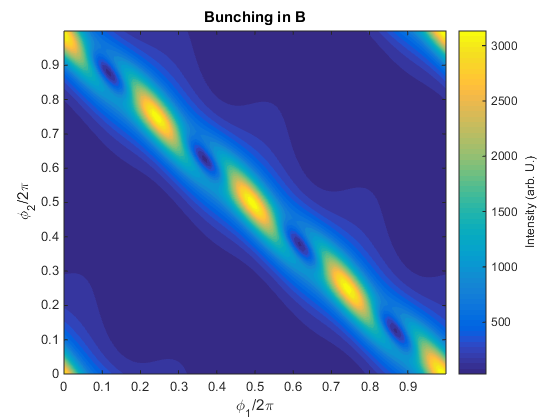
\includegraphics[width = \textwidth]{img/Bunching_B}
\caption{}
\end{subfigure}\,
\begin{subfigure}{0.49\textwidth}
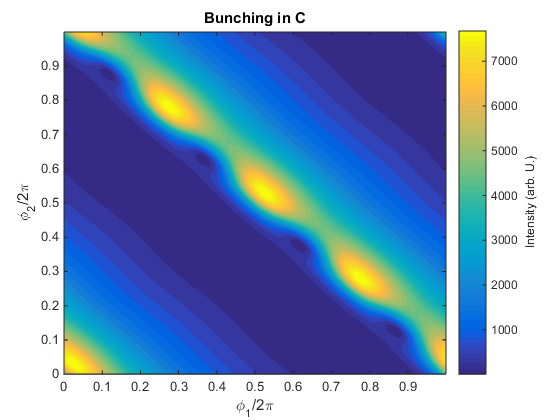
\includegraphics[width = \textwidth]{img/Bunching_C}
\caption{}
\end{subfigure}
\caption{Simulated probabilities (a) $|\beta_{bb}|^2$ and (b) $|\beta_{cc}|^2$ for the state $\ket{bb}$ and $\ket{cc}$ as a function of phases $\phi_1$ and $\phi_2$, not yet normalized. Credits to: Massimo Borghi}\label{bounchstates}
\end{figure}

\begin{figure}
\centering
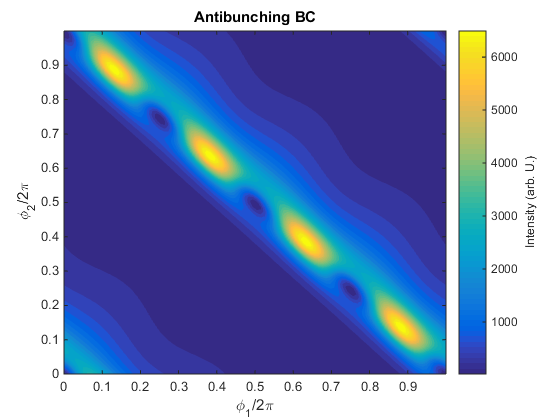
\includegraphics[width = .8\textwidth]{img/Antibunching_BC}
\caption{Simulated probability $|\beta_{bc}|^2$ for the state $\ket{bc}$ as a function of phases $\phi_1$ and $\phi_2$, not yet normalized. Credits to: Massimo Borghi}\label{antibounchstate}
\end{figure}

\chapter{Conclusion and further developments}
In this thesis I showed how entangled photon pairs are created inside a structure composed by two coupled resonators. Furthermore I showed how the output states change introducing two phases in the system. The final probabilities are a function of such phases and, as we analyzed in the last section, it is possible to decide where the photons exit. Exploiting this feature, there are two possibilities, by choosing the right phases a photon pair can exit either in B and with a similar probability in C, or the photon pair is splitted and one photon exit in B, while the other in C. This result has been obtained by computing the probabilities, but the calculation can go on, it is possibile to derive the power of the generated photons and also the rate. But the next important step is the experimental verification which is being performed by the nanoscience group of the University of Trento.\\
In this conclusion I want to dwell on entanglement, which in this work is almost not present. The generated photon pairs are energy and time entangled; the fact that the energy is entangled can be seen from equation \eqref{conservationenergy} which express the conservation of energy of the generated photon. The sum of the frequencies of the generated photons is fixed, so if a photon has a determined frequency, the frequency of the other one is determined. The frequency is linked to energy by the Planck's constant $E = \hbar \omega$, so speaking about photon frequency is to speak about photon energy. The time entanglement is trickier to see: for this it is necessary to perform coincidence measurements. From the photodetection it can be seen that there is zero delay between the photons' arrival, this means that the photons are emitted at the same time.